\documentclass[a4paper,11pt]{article}

\usepackage{hyperref}
\usepackage[landscape]{geometry}
\usepackage{fullpage}
\usepackage{multicol}
\usepackage{graphicx}
\usepackage{xspace}
\input{csvers}

\pagestyle{empty}

\setlength\columnseprule{0.4pt}
\addtolength\columnsep{2pt}

\newcommand{\refword}[1]{\texttt{$\bullet$ \bf{#1}}}

\begin{document}

\begin{multicols*}{3}

\begin{center}
  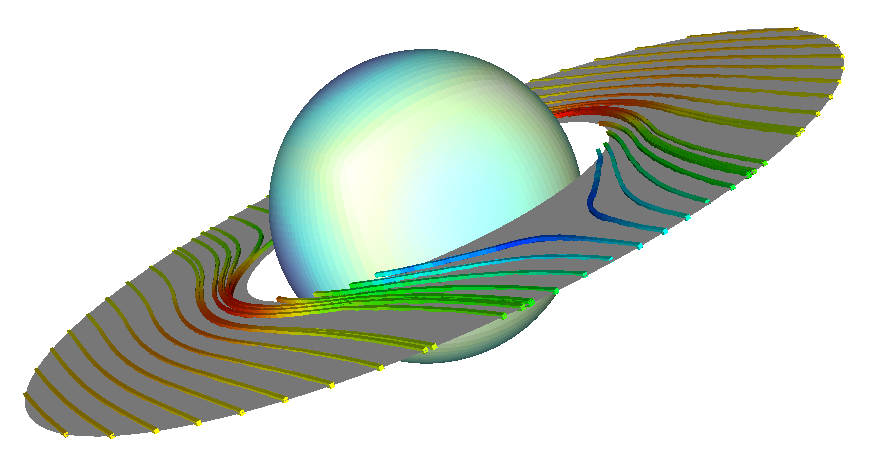
\includegraphics[width=5cm]{logocs}
  {\Large {\bf \CS~\verscs\\Quick reference card}}
\end{center}

% User scripts
% ------------

\section*{User scripts}

All \CS commands are available under a single script: \texttt{code\_saturne}.
Here below are the most useful commands for a \CS user from the study
creation to the post-processing. Complete information for each
\texttt{command} can be obtained by typing:\\
\texttt{code\_saturne <command> --help}.\\

\refword{info}\\
Get information on \CS. Open the documentation (user, theory,
tutorial).\\
\textit{e.g.} \texttt{code\_saturne info --guide=\emph{user}}\\

\refword{config}\\
Get information on the configuration and installation of \CS.\\
\textit{e.g.} \texttt{code\_saturne config}\\

\refword{create}\\
Create a \CS template study or case.\\
\textit{e.g.} \texttt{code\_saturne create --nogui --study=\emph{test}}\\

\refword{gui}\\
Launch \CS graphical user interface.\\
\textit{e.g.} \texttt{code\_saturne gui --file=\emph{xmlfile}}\\

\refword{check\_mesh}\\
Check the mesh quality.\\
\textit{e.g.} \texttt{code\_saturne check\_mesh -m \emph{mesh}}\\

\refword{compile}\\
Create a specific solver executable when some user subroutines are
present.\\
\textit{e.g.} \texttt{code\_saturne compile --test}\\

\refword{plot\_probes}\\
Wrapper around XmGrace for plotting probes monitoring.\\
\textit{e.g.} \texttt{code\_saturne plot\_probes \emph{VitesseX.hst}}

% User subroutines
% ----------------

\section*{Main user subroutines}

Here below are the most useful user subroutines to run a standard
simulation. Some of them are useless if the graphical user interface
is used.\\

\refword{usini1.f90}\\
Initialization of the main keywords.\\

\refword{usclim.f90}\\
Management of the boundary conditions.\\

\refword{usphyv.f90}\\
Management of the variable physical properties.\\

\refword{usiniv.f90}\\
Non-standard initialization of the variables.\\

\refword{usproj.f90}\\
User project files.\\

\refword{uskpdc.f90}\\
Management of the head loss.\\

\refword{usts**.f90}\\
User source terms related subroutines.\\

\refword{us*pst.f90}\\
Post-processing related subroutines.\\

% Main variables
% --------------

%\section*{Main variables}

% Practical information
% ---------------------

\section*{Practical information}

\url{http://www.code-saturne.org}\\

Related software:\\
\url{http://www.syrthes.org}\\
\url{http://www.code-aster.org}\\
\url{http://www.salome-platform.org}

\begin{center}
  
\includegraphics[width=2cm]{logoedf}
\end{center}

\end{multicols*}

\end{document}
